\section{ЧАСТЬ 1}

\begin{lstlisting}[caption=Текст программы]
#include <linux/module.h>
#include <linux/init.h>
#include <linux/kernel.h>
#include <linux/sched.h>
#include <linux/init_task.h>

MODULE_LICENSE("GPL");
MODULE_AUTHOR("Alexander Stepanov");
MODULE_DESCRIPTION("BMSTU operating sysytems lab_03_01");

static int __init alex_module_init(void)
{
    printk(KERN_INFO "Module loaded\n");

    struct task_struct *task = &init_task;

    do
    {
        printk(KERN_INFO "%s -- %d, parent: %s -- %d\n",
            task->comm, task->pid, task->parent->comm, task->parent->pid);
    }
    while ((task = next_task(task)) != &init_task);

 
    printk(KERN_INFO "current: %s -- %d, parent: %s -- %d\n",
        current->comm,
        current->pid,
        current->parent->comm,
        current->parent->pid
    );

    return 0;
}

static void __exit alex_module_exit(void)
{
    printk(KERN_INFO "Module exited\n");
}

module_init(alex_module_init);
module_exit(alex_module_exit);
\end{lstlisting}

\begin{figure}[H]
    \centering
    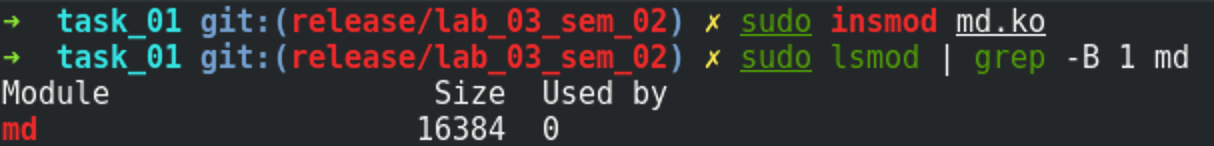
\includegraphics[scale=0.8]{img/part_01/insmod.png}
    \caption{Загрузка модуля}
\end{figure}

\begin{figure}[H]
    \centering
    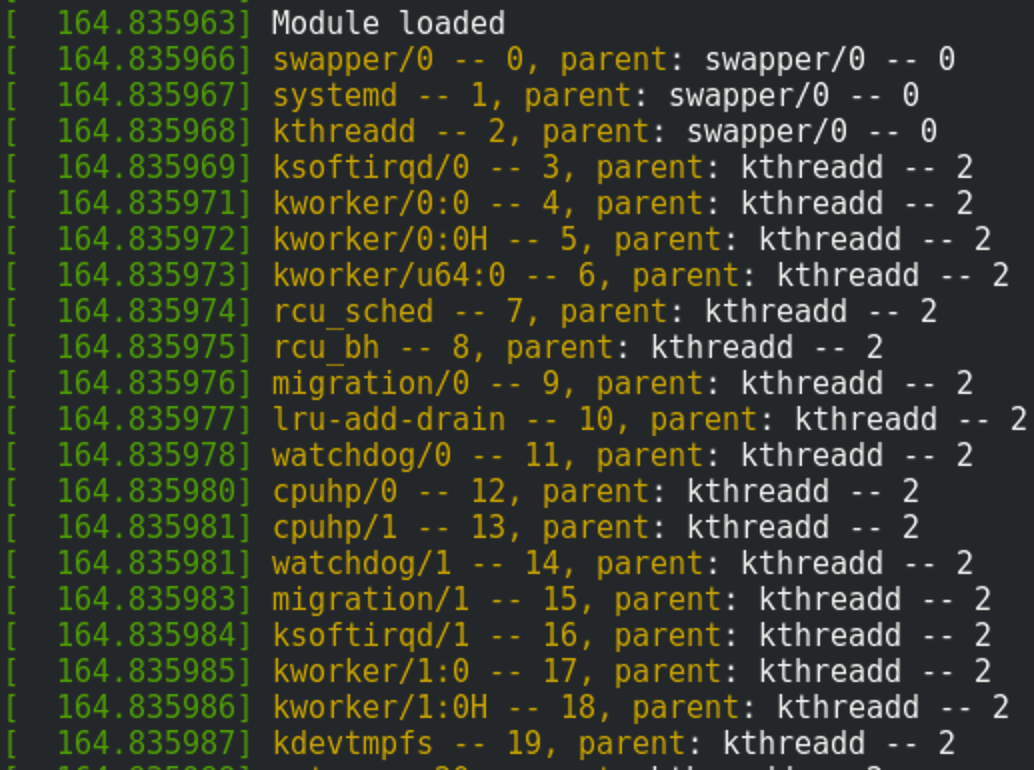
\includegraphics[scale=1]{img/part_01/dmesg_01.png}
    \caption{Вывод dmesg (часть 1)}
\end{figure}

\begin{figure}[H]
    \centering
    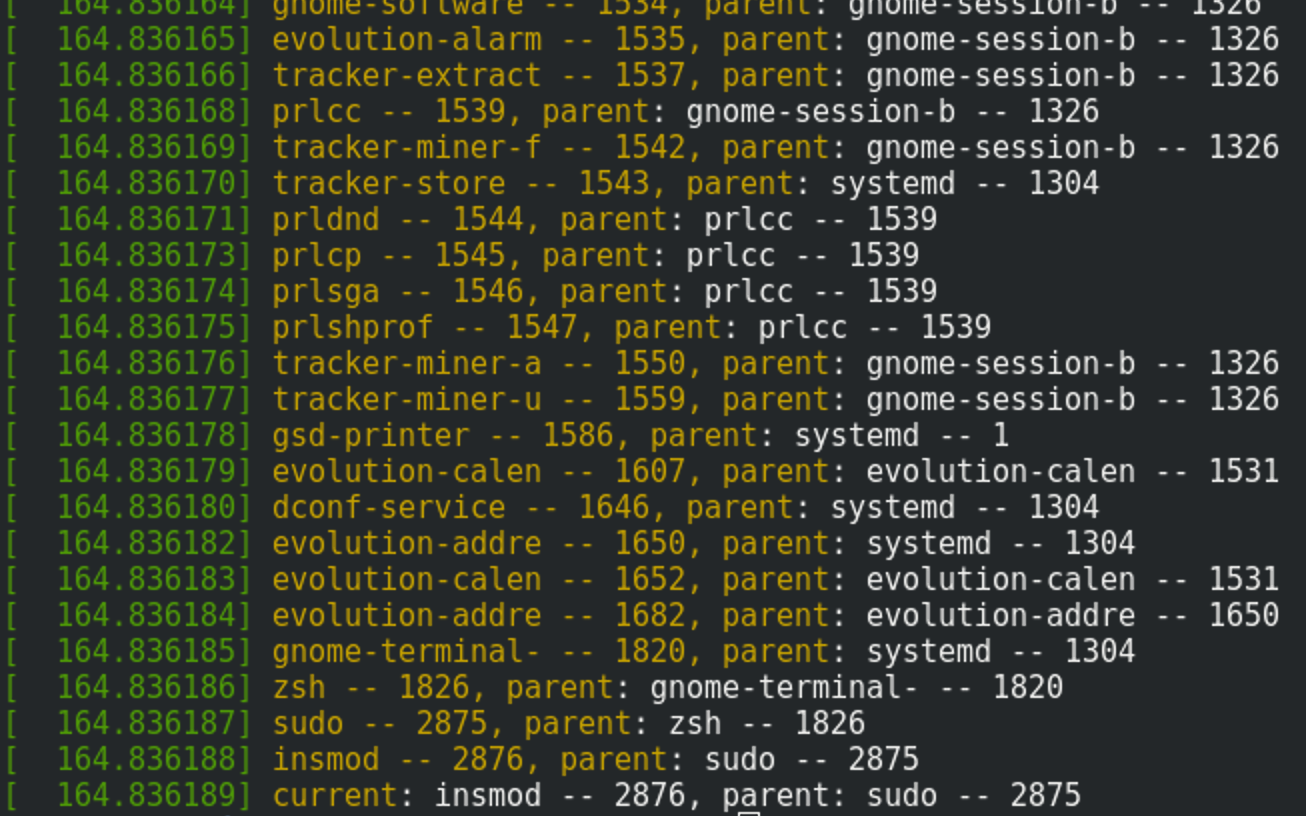
\includegraphics[scale=0.8]{img/part_01/dmesg_02.png}
    \caption{Вывод dmesg (часть 2)}
\end{figure}

\begin{figure}[H]
    \centering
    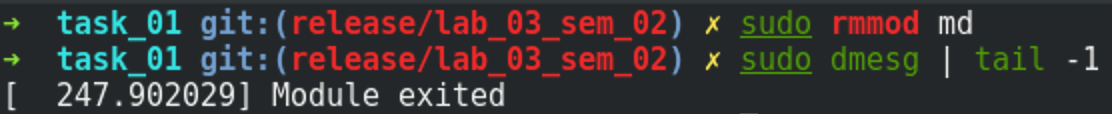
\includegraphics[scale=0.9]{img/part_01/rmmod.png}
    \caption{Выгрузка модуля}
\end{figure}

\section{ЧАСТЬ 2}

\begin{lstlisting}[caption=md1.c]
#include <linux/init.h> 
#include <linux/module.h> 
#include "md.h" 

MODULE_LICENSE("GPL"); 
MODULE_AUTHOR("Alexander Stepanov"); 

char* md1_str_data = "Привет мир!";
int md1_int_data = 42;

extern char* md1_get_str(int n) 
{ 
	printk( "+ md1: md1_get_str() called!\n" ); 
	switch (n)
	{
	case 1:
		return "Hello world!\n";
		break;
	case 2:
		return "Привет Мир!\n";
		break;
	default:
		return "Передайте 1 для получения английского сообщения"
            "или 2 для получения русского.\n";
		break;
	}
} 

extern int md1_factorial(int n) 
{ 
	int i, ans;
	ans = 1;
		
	printk( "+ md1: md1_factorial() called!\n" ); 
	for (i = 2; i <= n; i++) ans *= i;
	
	return ans;
}

/* экспортируем данные */
EXPORT_SYMBOL(md1_str_data); 
EXPORT_SYMBOL(md1_int_data); 
/* экспортируем функции */
EXPORT_SYMBOL(md1_get_str); 
EXPORT_SYMBOL(md1_factorial); 


static int __init md_init( void ) 
{ 
   printk( "+ md1: module md1 start!\n" ); 
   return 0; 
}

static void __exit md_exit( void ) 
{ 
   printk( "+ md1: module md1 unloaded!\n" ); 
} 

module_init( md_init ); 
module_exit( md_exit ); 
\end{lstlisting}

\begin{lstlisting}[caption=md.h]
extern char* md1_str_data;
extern int md1_int_data;
extern char* md1_get_str(int n);
extern int md1_factorial(int n);
\end{lstlisting}

\begin{lstlisting}[caption=md2.c]
#include <linux/init.h> 
#include <linux/module.h> 
#include "md.h" 

MODULE_LICENSE("GPL"); 
MODULE_AUTHOR("Alexander Stepanov"); 

static int __init md_init( void ) 
{ 
   printk( "+ md2: module md2 start!\n" ); 
   printk( "+ md2: Число экспортированное из md1 : %d\n", md1_int_data ); 
   printk( "+ md2: Строка экспортированная из md1 : %s\n", md1_str_data ); 
   printk( "+ md2: Результат работы функции md1_get_str(0) : %s\n",
    md1_get_str(0) );
   printk( "+ md2: Результат работы функции md1_get_str(1) : %s\n",
    md1_get_str(1) );
   printk( "+ md2: Результат работы функции md1_get_str(2) : %s\n",
    md1_get_str(2) );
   printk( "+ md2: Результат работы функции md1_factorial(4) : %d\n",
    md1_factorial(4) );  
   return 0; 
} 

static void __exit md_exit( void ) 
{ 
   printk( "+ md2: module md2 unloaded!\n" ); 
} 

module_init( md_init ); 
module_exit( md_exit );
\end{lstlisting}

\begin{lstlisting}[caption=md3.c]
#include <linux/init.h> 
#include <linux/module.h> 
#include "md.h" 

MODULE_LICENSE("GPL"); 
MODULE_AUTHOR("Alexander Stepanov"); 

static int __init md_init( void ) 
{ 
   printk("+ md3: module md3 start!\n"); 
   printk("+ md3: Число экспортированное из md1 : %d\n", md1_int_data); 
   printk("+ md3: Строка экспортированная из md1 : %s\n", md1_str_data); 
   printk("+ md3: Результат работы функции md1_get_str(0) : %s\n",
    md1_get_str(0));
   printk("+ md3: Результат работы функции md1_get_str(1) : %s\n",
    md1_get_str(1));
   printk("+ md3: Результат работы функции md1_get_str(2) : %s\n",
    md1_get_str(2));
   printk("+ md3: Результат работы функции md1_factorial(4) : %d\n",
    md1_factorial(4));
   return -1; 
} 

module_init( md_init ); 
\end{lstlisting}

В данных модулях продемострирована работа экспортируемых данных и функций. Модуль md1 экспортирует переменные md1\_str\_data и md1\_int\_data, которые импортируют модули md2 и md3. Поскольку md2 и md3 импортируют данные из модуля md, то они не могут быть загружены до загрузки модуля md1, что можно увидеть на рисунке \ref{img:incorrect_insmod}.

\begin{figure}[H]
    \centering
    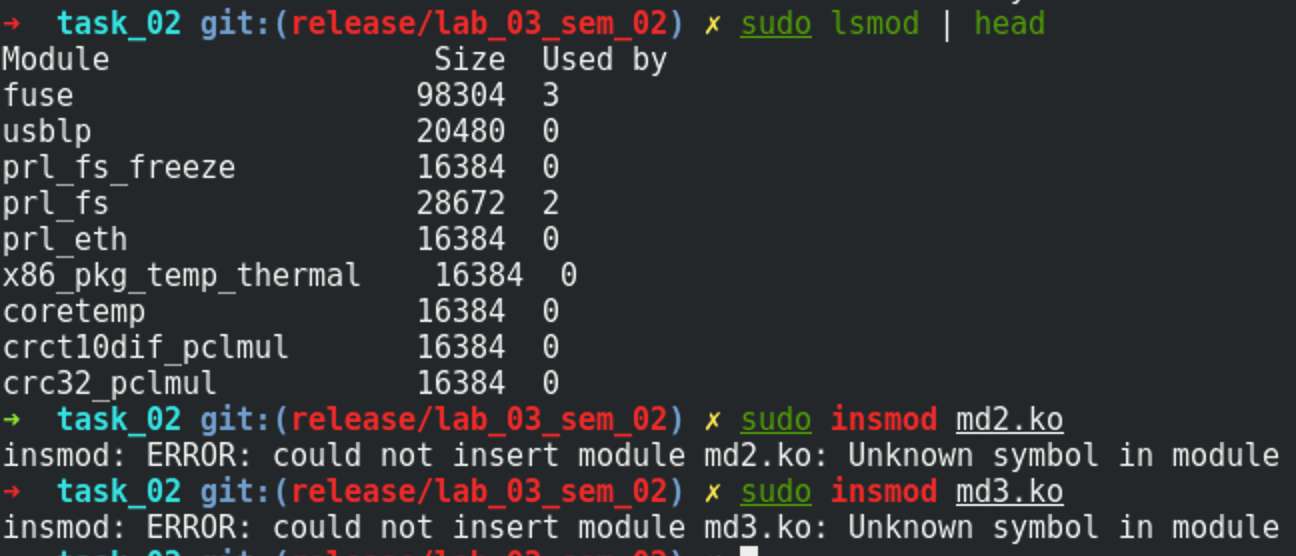
\includegraphics[scale=0.7]{img/part_02/incorrect_insmod.png}
    \caption{Попытка загрузить md2 и md3 до md1}
    \label{img:incorrect_insmod}
\end{figure}

Если же загрузить сначала модуль, который экспортирует данные, то все модули загрузятся (кроме md3, при инициализации которого возращается -1) (Рисунок \ref{img:insmod}).

\begin{figure}[H]
    \centering
    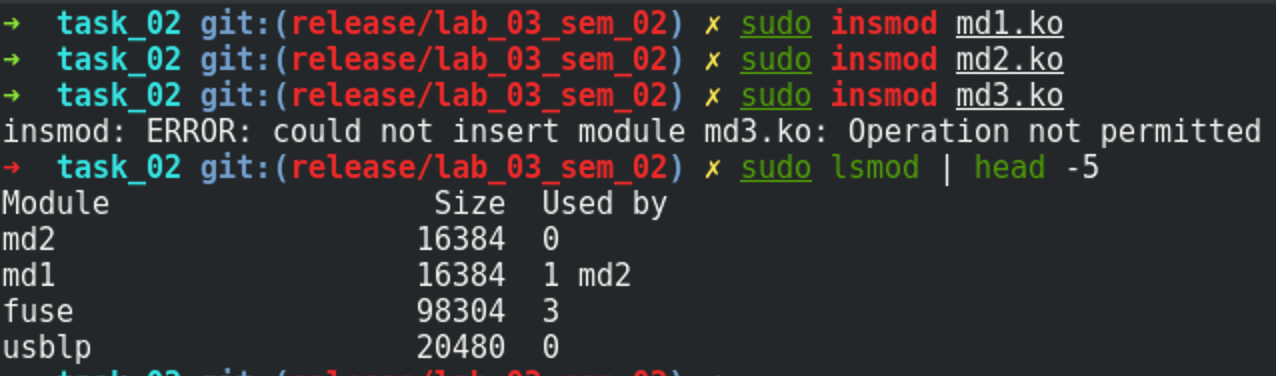
\includegraphics[scale=0.7]{img/part_02/insmod.png}
    \caption{Попытка загрузка модулей}
    \label{img:insmod}
\end{figure}

\begin{figure}[H]
    \centering
    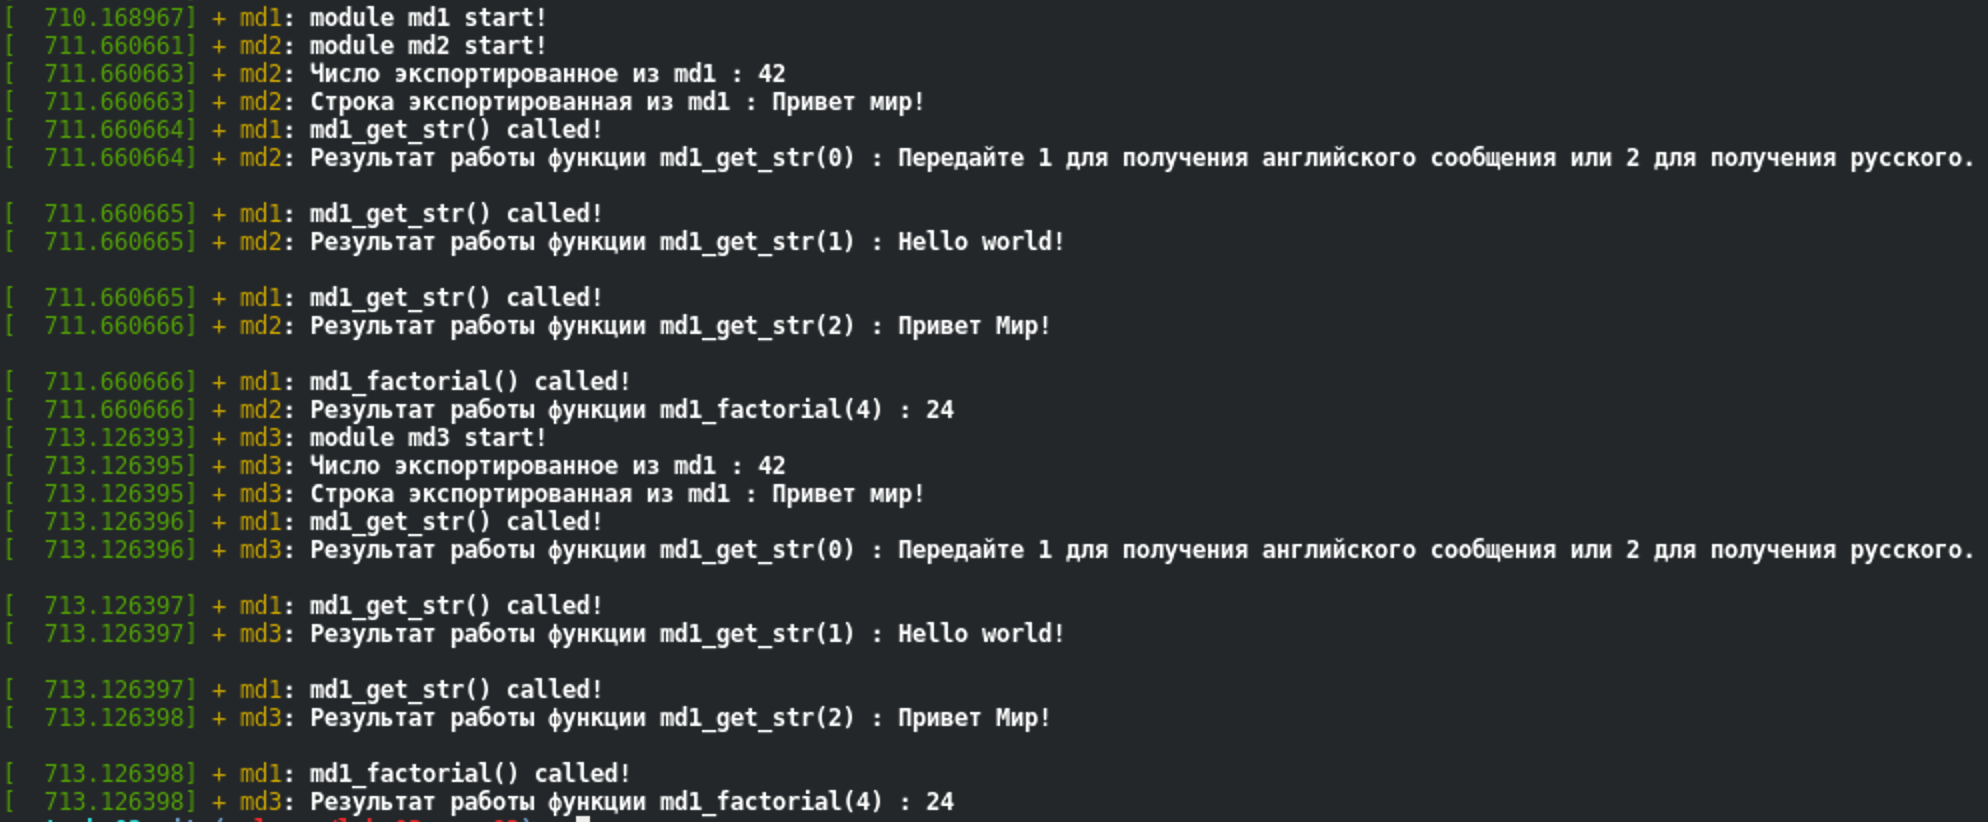
\includegraphics[scale=0.5]{img/part_02/dmesg.png}
    \caption{Вывод dmesg}
\end{figure}

В выводе команды lsmod можно увидеть, что модуль md1 используется модулем md2. Пока модуль md1 используется другим модулем, его нельзя выгрузить, что видно на рисунке \ref{img:incorrect_rmmod}.

\begin{figure}[H]
    \centering
    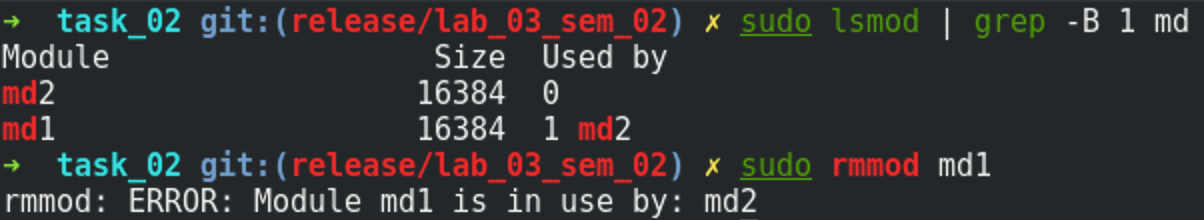
\includegraphics[scale=0.8]{img/part_02/incorrect_rmmod.png}
    \caption{Попытка выгрузить md1 до md2}
    \label{img:incorrect_rmmod}
\end{figure}

Если сначала выгрузить модуль md2, который импортирует данные, то можно выгрузить и md1 (Рисунок \ref{img:rmmod}).

\begin{figure}[H]
    \centering
    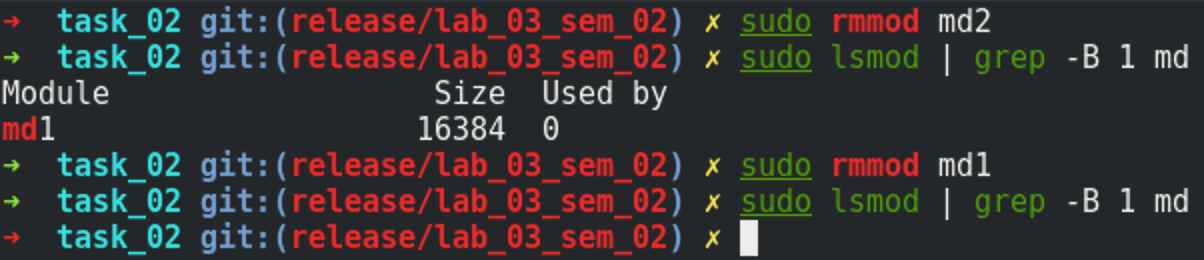
\includegraphics[scale=0.8]{img/part_02/rmmod.png}
    \caption{Выгрузка модулей}
    \label{img:rmmod}
\end{figure}
